% !TEX root = smc_bandits.tex
We simulate the following two-armed, contextual ($x_t\in\Real^2, \forall t$), linear Gaussian bandit:
\begin{equation}
\text{Scenario A}
\begin{cases}
	\vspace*{1ex}
	p(\theta_{t,a=0}|\theta_{t-1,a=0}): \\ \vspace*{1ex}
	\hspace*{10ex}\begin{pmatrix}
	\theta_{t,a=0,0}\\
	\theta_{t,a=0,1}\\
	\end{pmatrix} = \begin{pmatrix}
	0.9 & -0.1 \\
	-0.1 & 0.9 \\
	\end{pmatrix} \begin{pmatrix}
	\theta_{t-1,a=0,0}\\
	\theta_{t-1,a=0,1}\\
	\end{pmatrix} + \epsilon_{a=0} \;, \\ \vspace*{1ex}
	\hspace*{40ex} \text{where } \;  \epsilon_{a=0} \sim \N{\epsilon|0,0.01 \cdot\mathrm{I}},\\
	
	\vspace*{1ex}
	p(\theta_{t,a=1}|\theta_{t-1,a=1}): \\ \vspace*{1ex}
	\hspace*{10ex}\begin{pmatrix}
	\theta_{t,a=1,0}\\
	\theta_{t,a=1,1}\\
	\end{pmatrix} = \begin{pmatrix}
	0.9 & 0.1 \\
	0.1 & 0.9 \\
	\end{pmatrix} \begin{pmatrix}
	\theta_{t-1,a=1,0}\\
	\theta_{t-1,a=1,1}\\
	\end{pmatrix} + \epsilon_{a=1} \;, \\ \vspace*{1ex}
	\hspace*{40ex} \text{where } \;  \epsilon_{a=1} \sim \N{\epsilon|0,0.01 \cdot\mathrm{I}},\\
	
	p_a(Y|x,\theta_{t,a})=\N{Y|x^\top \theta_{t,a}, \sigma_a^2} \;.
\end{cases}
\label{eq:linear_mixing_dynamics_a}
\end{equation}

\begin{equation}
\text{Scenario B}
\begin{cases}
	\vspace*{1ex}
	p(\theta_{t,a=0}|\theta_{t-1,a=0}): \\ \vspace*{1ex}
	\hspace*{10ex}\begin{pmatrix}
	\theta_{t,a=0,0}\\
	\theta_{t,a=0,1}\\
	\end{pmatrix} = \begin{pmatrix}
	0.5 & 0.0 \\
	0.0 & 0.5 \\
	\end{pmatrix} \begin{pmatrix}
	\theta_{t-1,a=0,0}\\
	\theta_{t-1,a=0,1}\\
	\end{pmatrix} + \epsilon_{a=0} \;, \\ \vspace*{1ex}
	\hspace*{40ex} \text{where } \;  \epsilon_{a=0} \sim \N{\epsilon|0,0.01 \cdot\mathrm{I}},\\
	
	\vspace*{1ex}
	p(\theta_{t,a=1}|\theta_{t-1,a=1}): \\ \vspace*{1ex}
	\hspace*{10ex}\begin{pmatrix}
	\theta_{t,a=1,0}\\
	\theta_{t,a=1,1}\\
	\end{pmatrix} = \begin{pmatrix}
	0.9 & 0.1 \\
	0.1 & 0.9 \\
	\end{pmatrix} \begin{pmatrix}
	\theta_{t-1,a=1,0}\\
	\theta_{t-1,a=1,1}\\
	\end{pmatrix} + \epsilon_{a=1} \;, \\ \vspace*{1ex}
	\hspace*{40ex} \text{where } \;  \epsilon_{a=1} \sim \N{\epsilon|0,0.01 \cdot\mathrm{I}}, \\
	
	p_a(Y|x,\theta_{t,a})=\N{Y|x^\top \theta_{t,a}, \sigma_a^2} \;.
\end{cases}
\label{eq:linear_mixing_dynamics_b}
\end{equation}
 
The expected rewards driven by the dynamics of Equations~\eqref{eq:linear_mixing_dynamics_a} and~\eqref{eq:linear_mixing_dynamics_b} change over time,
inducing switches on the identity of the optimal arm.
%
For instance, for a given realization of Scenario A shown in Figure~\ref{fig:linear_mixing_dynamics_a_gaussian},
there is an optimal arm swap between time-instants $t=(300, 550)$, with arm 1 becoming the optimal for all $t\geq600$;
for a realization of Scenario B illustrated in Figure~\ref{fig:linear_mixing_dynamics_b_gaussian},
there is an optimal arm change around $t=100$, a swap around $t=600$,
with arm 1 becoming optimal again after $t\geq1600$.

Empirical results for SMC-based Bayesian policies in scenarios described by Equations~\eqref{eq:linear_mixing_dynamics_a} and~\eqref{eq:linear_mixing_dynamics_b}
are shown in Figures~\ref{fig:dynamic_bandits_linearGaussian_dknown} and \ref{fig:dynamic_bandits_linearGaussian_dunknown}.

% Linear Gaussian, known parameters
\begin{figure}[!h]
	\centering
	\begin{subfigure}[b]{0.45\textwidth}
		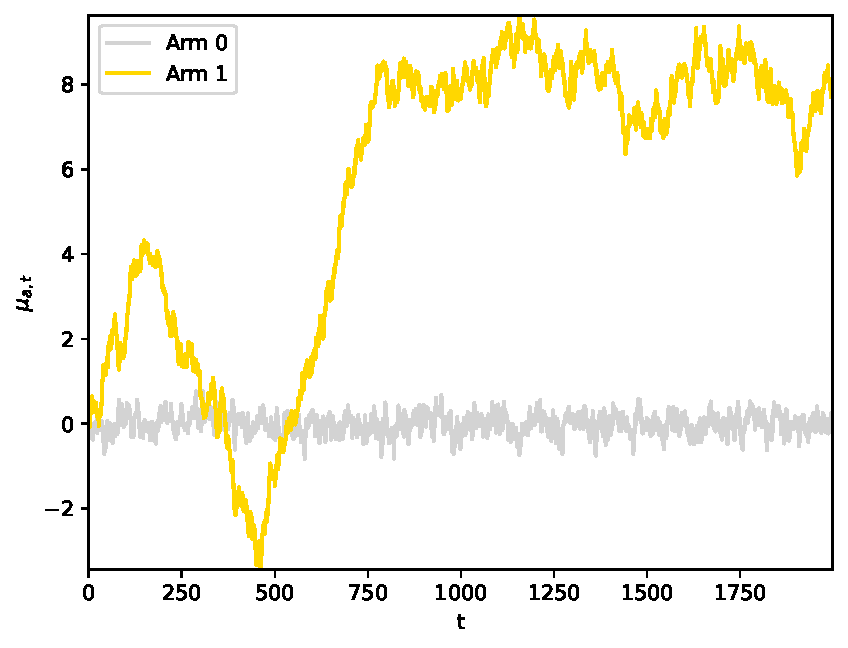
\includegraphics[width=\textwidth]{./fods_figs/dynamic/linearGaussian/dynamics_a}
		\caption{Expected per-arm rewards over time for Scenario A in Equation~\eqref{eq:linear_mixing_dynamics_a}.}
		\label{fig:linear_mixing_dynamics_a_gaussian}
	\end{subfigure}\qquad
	\begin{subfigure}[b]{0.45\textwidth}
		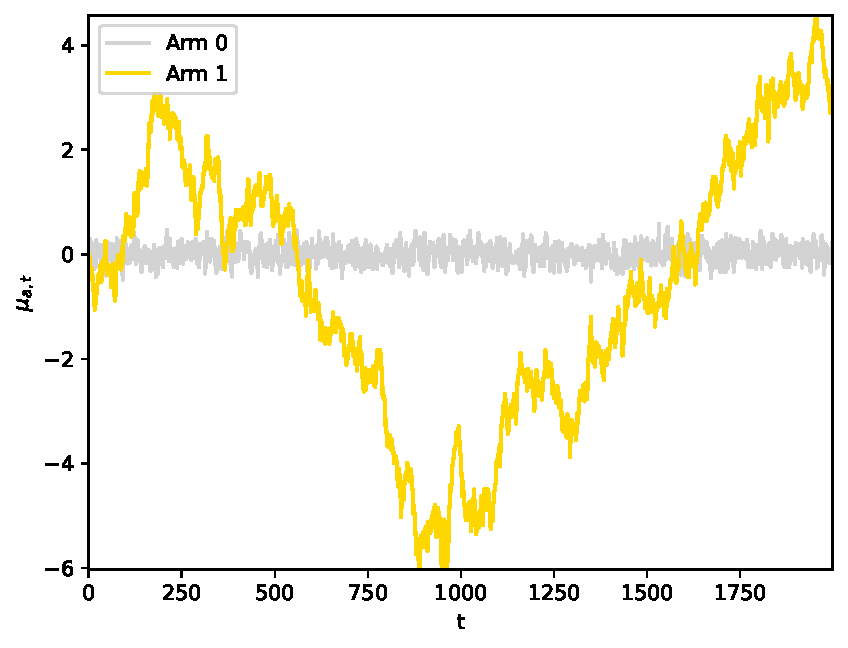
\includegraphics[width=\textwidth]{./fods_figs/dynamic/linearGaussian/dynamics_b}
		\caption{Expected per-arm rewards over time for Scenario B in Equation~\eqref{eq:linear_mixing_dynamics_a}.}
		\label{fig:linear_mixing_dynamics_b_gaussian}
	\end{subfigure}
	
	\begin{subfigure}[b]{0.47\textwidth}
		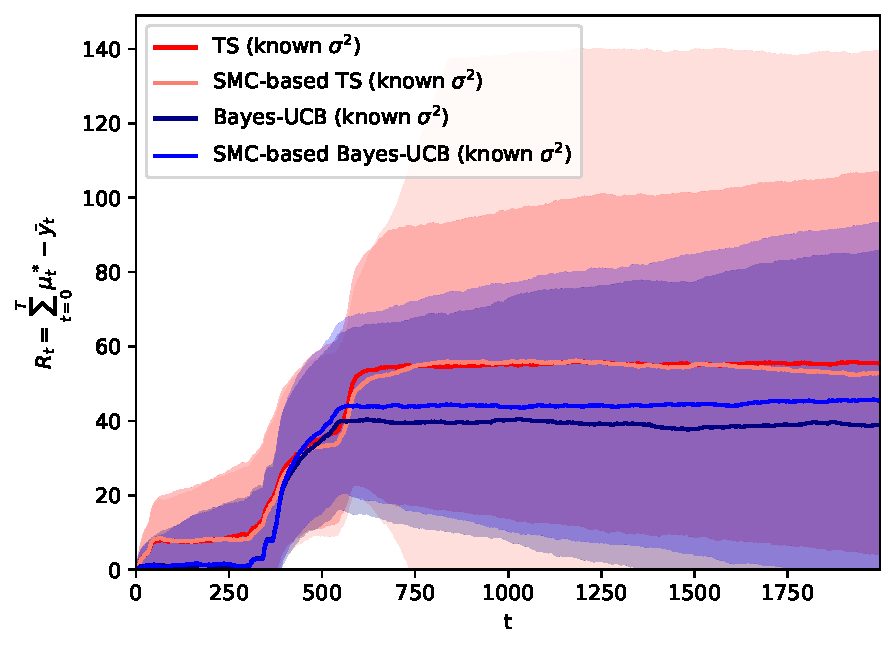
\includegraphics[width=\textwidth]{./fods_figs/dynamic/linearGaussian/a_M2000_cumulative_regret_dknown_knownsigma}
		\caption{Cumulative regret for SMC-based Bayesian policies in scenario A: known dynamic parameters.}
		\label{fig:dynamic_bandits_linearGaussian_a_cstatic_dknown_knownsigma}
	\end{subfigure}\qquad
	\begin{subfigure}[b]{0.47\textwidth}
		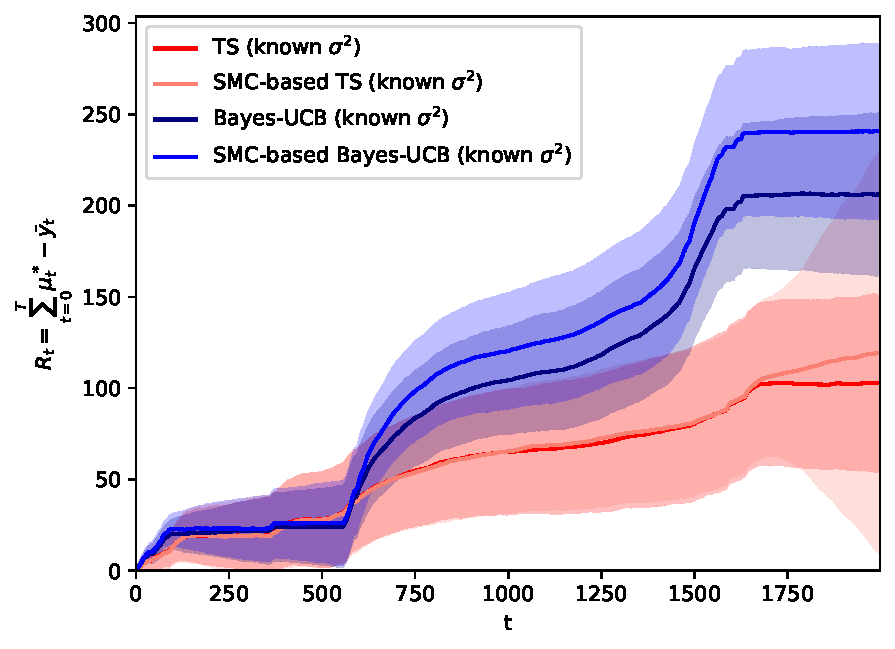
\includegraphics[width=\textwidth]{./fods_figs/dynamic/linearGaussian/b_M2000_cumulative_regret_dknown_knownsigma}
		\caption{Cumulative regret for SMC-based Bayesian policies in scenario B: known dynamic parameters.}
		\label{fig:dynamic_bandits_linearGaussian_b_cstatic_dknown_knownsigma}
	\end{subfigure}
	
	\caption{
		Mean regret (standard deviation shown as shaded region) in contextual, linear Gaussian bandit Scenarios A and B
		described in Equations~\eqref{eq:linear_mixing_dynamics_a}--\eqref{eq:linear_mixing_dynamics_b},
		when the bandit agent knows the latent dynamic parameterization.
		Notice how
		in Figures~\ref{fig:dynamic_bandits_linearGaussian_a_cstatic_dknown_knownsigma}--\ref{fig:dynamic_bandits_linearGaussian_b_cstatic_dknown_knownsigma}
		regret increases when the optimal arms swap
		(as shown in Figures~\ref{fig:linear_mixing_dynamics_a_gaussian}--\ref{fig:linear_mixing_dynamics_b_gaussian}).
		SMC-based policies successfully find the right exploration-exploitation tradeoff,
		with minimal additional regret incurred in comparison to their analytical alternatives. 
	}
	\label{fig:dynamic_bandits_linearGaussian_dknown}
\end{figure}

We study linear dynamics with Gaussian reward distributions with known parameters in Figure~\ref{fig:dynamic_bandits_linearGaussian_dknown},
of interest as it allows us to validate the SMC-based random measure in comparison to the optimal, closed-form posterior
---the Kalman filter~\cite{j-Kalman1960}---
under the assumption of known dynamic parameters.

We observe satisfactory cumulative regret performance in Figure~\ref{fig:dynamic_bandits_linearGaussian_dknown}:
\ie SMC-based Bayesian agents' cumulative regret is sublinear.
Policies that compute and use SMC random measure posteriors
incur in minimal regret loss 
in comparison to the optimal Kalman filter-based agent.
Namely, the shape of the regret curves of \textit{TS} and \textit{SMC-based TS}
(\textit{Bayes-UCB} and \textit{SMC based Bayes-UCB}, respectively) in Figure~\ref{fig:dynamic_bandits_linearGaussian_dknown} is equivalent,
with minimal differences in average cumulative regret when compared to the volatility across realizations.
Importantly, all policies are able to adapt to the changes over time of the identify of the optimal arm. 

We illustrate in Figure~\ref{fig:dynamic_bandits_linearGaussian_dunknown}
a more realistic scenario, where the dynamic parameterization is unknown to the bandit agent.

We observe in Figures~\ref{fig:dynamic_bandits_linearGaussian_a_cstatic_dknown_unknownsigma}--\ref{fig:dynamic_bandits_linearGaussian_b_cstatic_dknown_unknownsigma} that,
in the case of unknown reward variances ($\sigma_a^2, \forall a)$,
SMC-based policies perform comparably well.
In these cases,
the agents' reward model is not Gaussian,
but Student-t distributed, as per the marginalized posterior in Equation~\eqref{eq:t_posterior_mean}.
The regret loss associated with the uncertainty about $\sigma_a^2$ is minimal for SMC-based Bayesian agents,
and does not hinder the ability of the proposed SMC-based policies
to find the right exploration-exploitation balance:
\ie regret is sublinear, and the agents adapt to switches in the identity of the optimal arm.

We illustrate in Figures~\ref{fig:dynamic_bandits_linearGaussian_a_cstatic_dunknown}--\ref{fig:dynamic_bandits_linearGaussian_b_cstatic_dunknown}
the most realistic, yet challenging, non-stationary contextual Gaussian bandit case:
one where none of the parameters of the model are known.
In this case, the agent must sequentially learn both the underlying dynamics ($L_a,\Sigma_a; \forall a$)
and the conditional reward function's variance ($\sigma_a^2, \forall a)$,
in order to infer the posterior distribution over the latent, time-varying sufficient statistics of interest,
to enable informed sequential decision making.

Cumulative regret results in Figures~\ref{fig:dynamic_bandits_linearGaussian_a_cstatic_dunknown}--\ref{fig:dynamic_bandits_linearGaussian_b_cstatic_dunknown}
showcase a regret performance loss due to the need to learn all these unknown parameters.
We observe noticeable (almost linear) regret increases when the dynamics of the parameters swap the identity of the optimal arm.
However, SMC-based Thompson sampling and Bayes-UCB agents are able to learn the evolution of the dynamic latent parameters,
and the corresponding time-varying expected rewards,
with enough accuracy to attain good exploration-exploitation balance:
\ie sublinear regret curves indicate the agent identified and played the optimal arm repeatedly.
Figure~\ref{fig:dynamic_bandits_linearGaussian_a_cstatic_dunknown} is clear evidence of the SMC-based agents' ability to recover from linear to no-regret regimes.

\begin{figure}[!h]
	\centering
	\begin{subfigure}[b]{0.45\textwidth}
		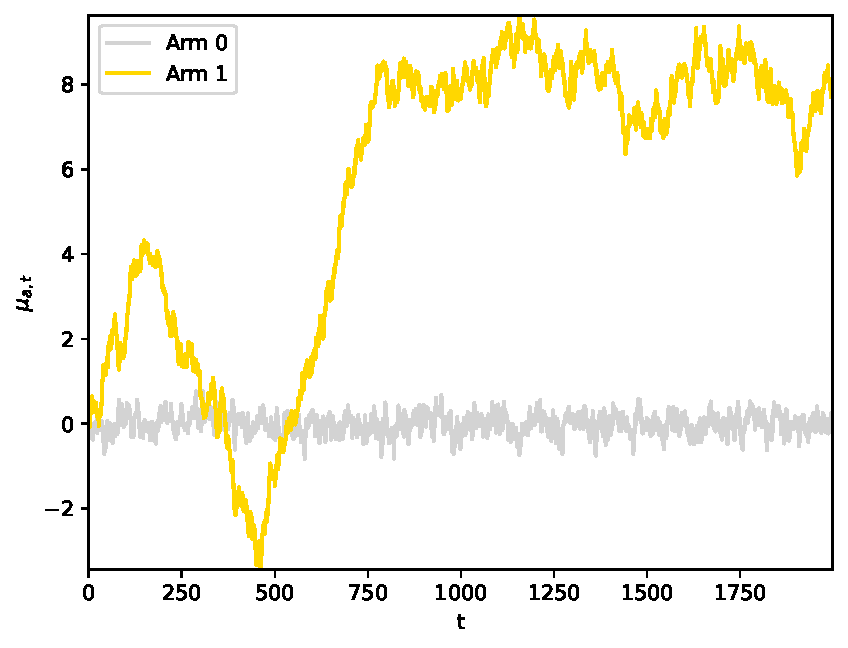
\includegraphics[width=\textwidth]{./fods_figs/dynamic/linearGaussian/dynamics_a}
		\caption{Expected per-arm rewards over time for Scenario A in Equation~\eqref{eq:linear_mixing_dynamics_a}.}
		\label{fig:linear_mixing_dynamics_a_gaussian_2}
	\end{subfigure}\qquad
	\begin{subfigure}[b]{0.45\textwidth}
		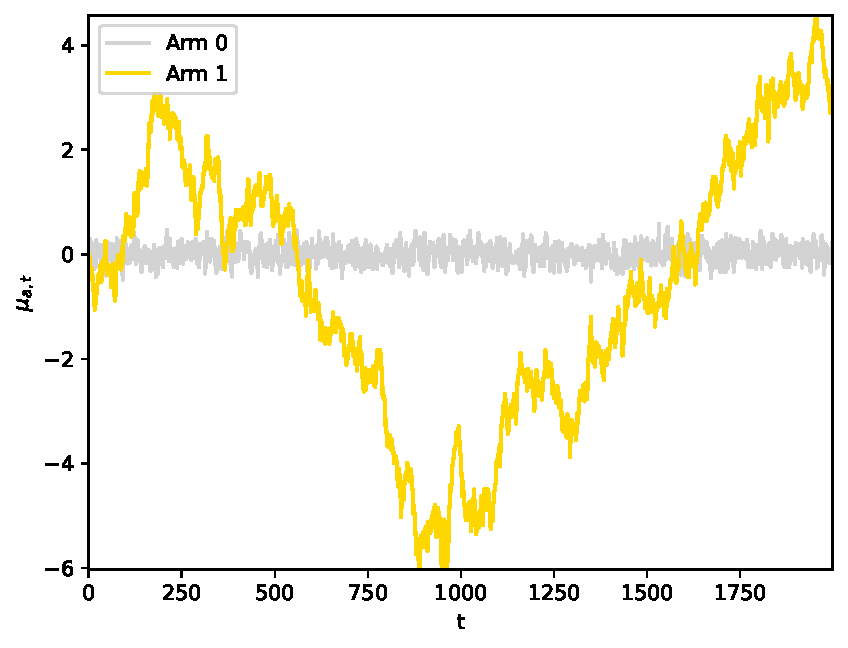
\includegraphics[width=\textwidth]{./fods_figs/dynamic/linearGaussian/dynamics_b}
		\caption{Expected per-arm rewards over time for Scenario B in Equation~\eqref{eq:linear_mixing_dynamics_a}.}
		\label{fig:linear_mixing_dynamics_b_gaussian_2}
	\end{subfigure}
	
	\begin{subfigure}[b]{0.47\textwidth}
		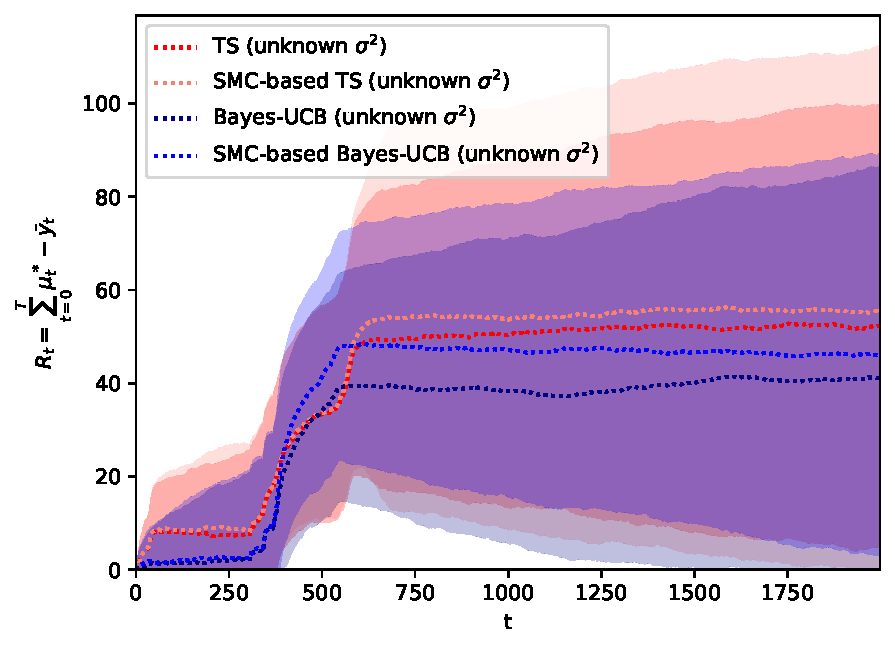
\includegraphics[width=\textwidth]{./fods_figs/dynamic/linearGaussian/a_M2000_cumulative_regret_dknown_unknownsigma}
		\caption{Cumulative regret for SMC-based Bayesian policies in scenario A: known dynamic parameters, unknown $\sigma_a, \forall a$.}
		\label{fig:dynamic_bandits_linearGaussian_a_cstatic_dknown_unknownsigma}
	\end{subfigure}\qquad
	\begin{subfigure}[b]{0.47\textwidth}
		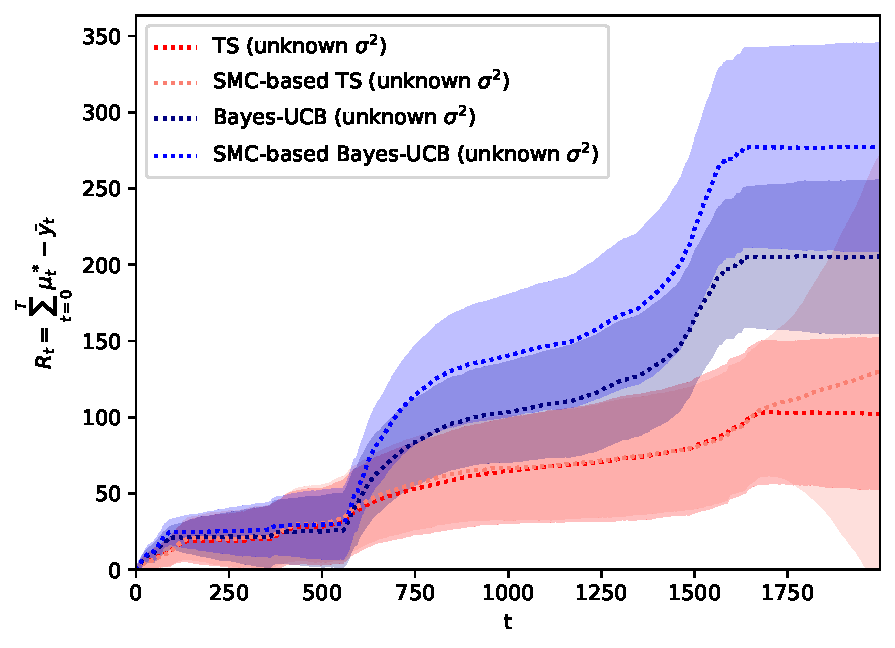
\includegraphics[width=\textwidth]{./fods_figs/dynamic/linearGaussian/b_M2000_cumulative_regret_dknown_unknownsigma}
		\caption{Cumulative regret for SMC-based Bayesian policies in scenario B: known dynamic parameters, unknown $\sigma_a, \forall a$.}
		\label{fig:dynamic_bandits_linearGaussian_b_cstatic_dknown_unknownsigma}
	\end{subfigure}
	
	\begin{subfigure}[b]{0.47\textwidth}
		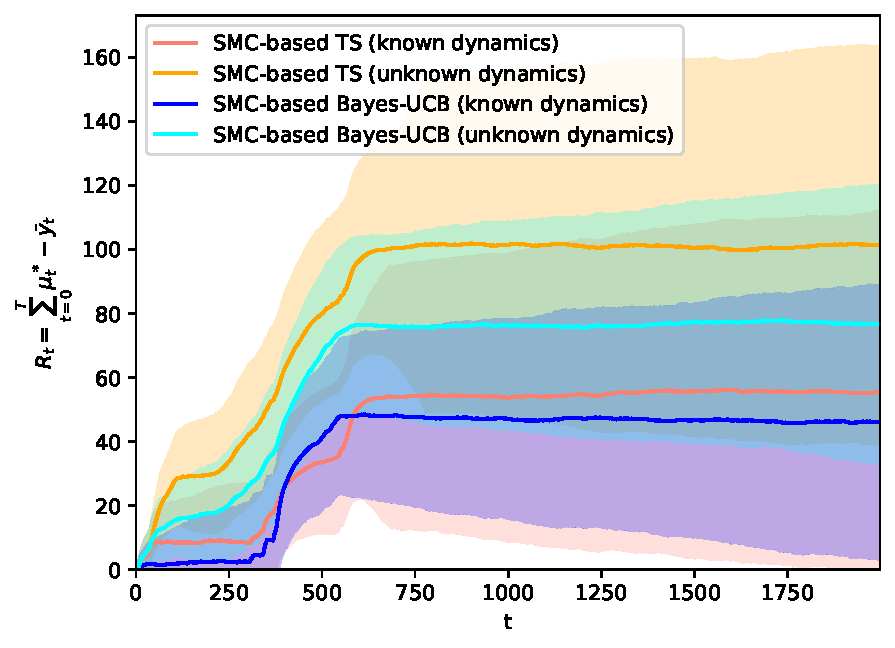
\includegraphics[width=\textwidth]{./fods_figs/dynamic/linearGaussian/a_M2000_cumulative_regret_dunknown}
		\caption{Cumulative regret for SMC-based Bayesian policies in scenario A: unknown dynamic parameters $L_a,\Sigma_a,\sigma_a^2, \forall a$.}
		\label{fig:dynamic_bandits_linearGaussian_a_cstatic_dunknown}
	\end{subfigure}\qquad
	\begin{subfigure}[b]{0.47\textwidth}
		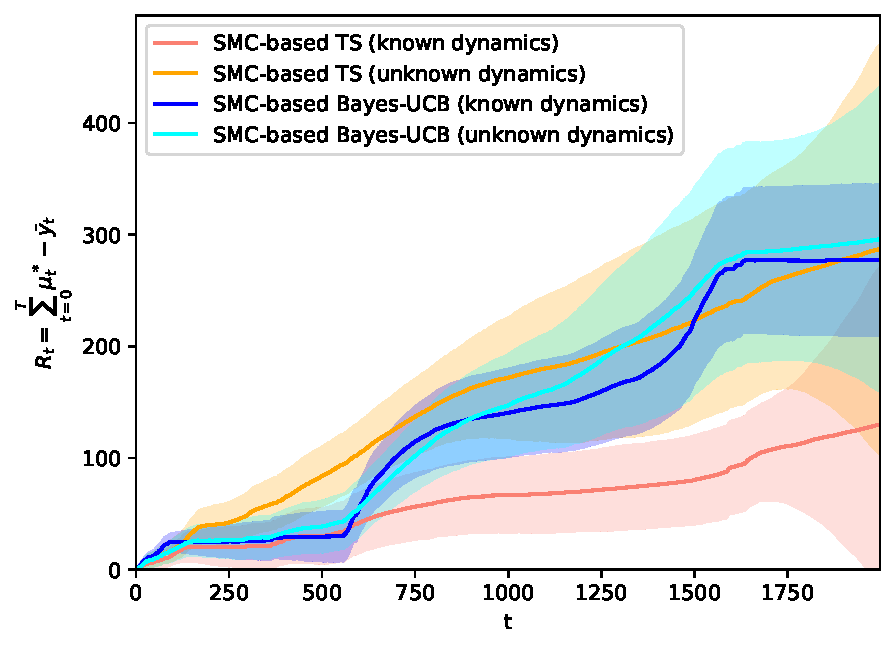
\includegraphics[width=\textwidth]{./fods_figs/dynamic/linearGaussian/b_M2000_cumulative_regret_dunknown}
		\caption{Cumulative regret for SMC-based Bayesian policies in scenario B: unknown dynamic parameters $L_a,\Sigma_a,\sigma_a^2, \forall a$.}
		\label{fig:dynamic_bandits_linearGaussian_b_cstatic_dunknown}
	\end{subfigure}
	\caption{
		Mean regret (standard deviation shown as shaded region) in contextual, linear Gaussian bandit Scenarios A and B
		described in Equations~\eqref{eq:linear_mixing_dynamics_a}--\eqref{eq:linear_mixing_dynamics_b},
		in the realistic setting of unknown dynamic parameters.
		Notice how
			in Figures~\ref{fig:dynamic_bandits_linearGaussian_a_cstatic_dknown_unknownsigma}--\ref{fig:dynamic_bandits_linearGaussian_b_cstatic_dunknown}
		the regret increases when the optimal arms swap
			(as shown in Figures~\ref{fig:linear_mixing_dynamics_a_gaussian_2}--\ref{fig:linear_mixing_dynamics_b_gaussian_2}).
		SMC-based policies find the right exploration-exploitation tradeoff even when the latent dynamic parameters are unknown.}
	\label{fig:dynamic_bandits_linearGaussian_dunknown}
\end{figure}
